% % % % % % % % % % % % % % % % % % % % % % % % % % % % % % % % % % % % % % I
\section{University Class Scheduling Problem (UCSP)}
\subsection{The Problem}

\begin{frame}{University Class Scheduling Problem}
  \begin{block}{The Problem}
    \textbf{U}niversity \textbf{C}lass \textbf{S}cheduling \textbf{P}roblem (UCSP)
    consists in finding valid \alert{class} assignations for \underline{all} the
    participants:
    \begin{itemize}
      \item Groups / Students
      \item Professors
    \end{itemize}
  \end{block}
  \begin{block}{Class}
    A class is an educational event, that is formed with purpose of studying
    some \alert{discipline}.
    \begin{columns}
      \begin{column}{4cm}
        \\Takes place
        \begin{itemize}
          \item in a \underline{classroom}
          \item on given \underline{day}
          \item during given \underline{time}
        \end{itemize}
      \end{column}
      \begin{column}{3cm}
        Links together
        \begin{itemize}
          \item a \underline{group} and
          \item a \underline{professor}
        \end{itemize}
      \end{column}
    \end{columns}

  \end{block}
\end{frame}

\begin{frame}
  \begin{columns}
    \begin{column}{4cm}
      \begin{block}{Schedule}
        The complete schedule consists of all the classes of all the participants,
        that can be seen as points in 5-dimensional space. It can be decomposed
        into a set of \alert{timetables}.
      \end{block}
    \end{column}
    \begin{column}{7cm}
        \resizeinput{\rootdir/img/ScheduleHypercube/GRPT-content.tikz}
    \end{column}
  \end{columns}
\end{frame}

\begin{frame}
  \begin{block}{Timetable}
    Timetable is projection of the schedule on the person/entity.
    It is a 2-dimensional table, that contains \underline{only} the classes
    of projection target.
  \end{block}
  \begin{columns}
    \begin{column}{.5\textwidth}
      \centering
      \begin{tabular}{|c||c|c|c|}
  \hline & Mon & Tue & $\cdots$ \\
  \hhline{|=#=|=|=|}
  08:30 -- 08:40 & x & & \\\hline
  08:40 -- 08:50 & x & & \\\hline
  08:50 -- 09:00 & x & & \\\hline
  $\vdots$\quad~--~\quad$\vdots$ & & & \\\hline
  09:50 -- 10:00 & x & & \\\hline
  10:00 -- 10:10 &   & & \\\hline
  10:10 -- 10:20 & y & & \\\hline
  10:20 -- 10:30 & y & & \\\hline
  $\vdots$\quad~--~\quad$\vdots$ & & & \\\hline
\end{tabular}

    \end{column}
    \begin{column}{.5\textwidth}
      \centering
      \begin{tabular}{|c||c|c|c|}
  \hline & Mon & Tue & $\cdots$ \\
  \hhline{|=#=|=|=|}
  08:30 -- 09:15 & x & & \\\hline
  09:25 -- 10:10 & x & & \\\hline
  10:30 -- 11:15 & y & & \\\hline
  11:25 -- 12:10 & y & & \\\hline
  Lunch          &   & & \\\hline
  13:25 -- 14:10 & z & & \\\hline
  14:20 -- 15:05 & z & & \\\hline
  15:25 -- 16:10 &   & & \\\hline
  $\vdots$\quad~--~\quad$\vdots$ & & & \\\hline
\end{tabular}

    \end{column}
  \end{columns}
  % \centering
  % \begin{tabular}{|c||c|c|c|c|c|c|}
  \hline & Mon & Tue & Wed & Thu & Fri & Sat \\
  \hhline{|=#=|=|=|=|=|=|}
  08:00 -- 08:30 & x & & & w & & \\\hline
  08:30 -- 09:00 & x & & & w & & \\\hline
  09:00 -- 09:30 & x & & & z & & \\\hline
  09:30 -- 10:00 & y & & & z & & \\\hline
  10:00 -- 10:30 & y & & & z & & \\\hline
  $\vdots$\quad~--~\quad$\vdots$ & & & & & & \\\hline
  21:00 -- 21:30 &   & & & & & \\\hline
  21:30 -- 22:00 &   & & & & & \\\hline
\end{tabular}

\end{frame}

% % % % % % % % % % % % % % % % % % % %
\subsection{Constraints}

\begin{frame}[label=constraints]{University Class Scheduling Constraints}
  \fbox{
    \begin{columns}[t]
      ~~Independent
      \begin{column}{.4\textwidth}
        \begin{block}{Class}
          \begin{itemize}
            \item Group need
            \item Professor can teach
            \item Classroom is suitable
          \end{itemize}
        \end{block}
      \end{column}
      \begin{column}{.4\textwidth}
        \begin{block}{Time}
          \begin{itemize}
            \item Classes non intersection
          \end{itemize}
        \end{block}
      \end{column}
    \end{columns}
  }
  \\[.7cm]
  \fbox{
    \begin{columns}[t]
      Personal
      \begin{column}{.4\textwidth}
        \begin{block}{Obligations}
          \begin{itemize}
            \item Personal \alert{strong} restrictions
          \end{itemize}
        \end{block}
      \end{column}
      \begin{column}{.4\textwidth}
        \begin{block}{Preferences}
          \begin{itemize}
            \item Personal \alert{weak} restrictions
          \end{itemize}
        \end{block}
      \end{column}
    \end{columns}
  }
\end{frame}

% % % % % % % % % % % % % % % % % % % % % % % % % % % % % % % % % % % % % % II
\section{Constraint Satisfaction Problem (CSP)}
% \subsection{CSP Definition}
% \subsection{CSP Examples}
% \subsection{CSP Solution Methods}

\begin{frame}{Constraint Satisfaction Problem}
  \begin{examples}
    \begin{columns}
      \begin{column}{.4\textwidth}
        \centering
        Queen moves/attacks\\ \medskip
        \resizeinput{\rootdir/img/NQueens/Restrictions-content.tikz}
      \end{column}
      \begin{column}{.6\textwidth}
        \centering
        \resizebox{\textwidth}{!}{%
        $\xi_2(\left<x_1,y_1\right>, \left<x_2,y_2\right>) =
            \begin{cases}
              0 & \mbox{if } \begin{cases}
                                &      x_1 = x_2  \lor y_1 = y_2 \\
                                \lor~& x_1 = y_2 \land x_2 = y_1 \\
                                \lor~& x_1-y_1 = x_2-y_2\\
                                \lor~& x_1+y_1 = x_2+y_2
                             \end{cases} \\
             1 & \text{otherwise}
            \end{cases}
        $}%
      \end{column}
    \end{columns}
  \end{examples}
\end{frame}

\begin{frame}{Constraint Satisfaction Problem}
  \begin{examples}
    \begin{columns}[t]
      \begin{column}{.4\textwidth}
        \centering
        Part of Central Europe\\ \medskip
        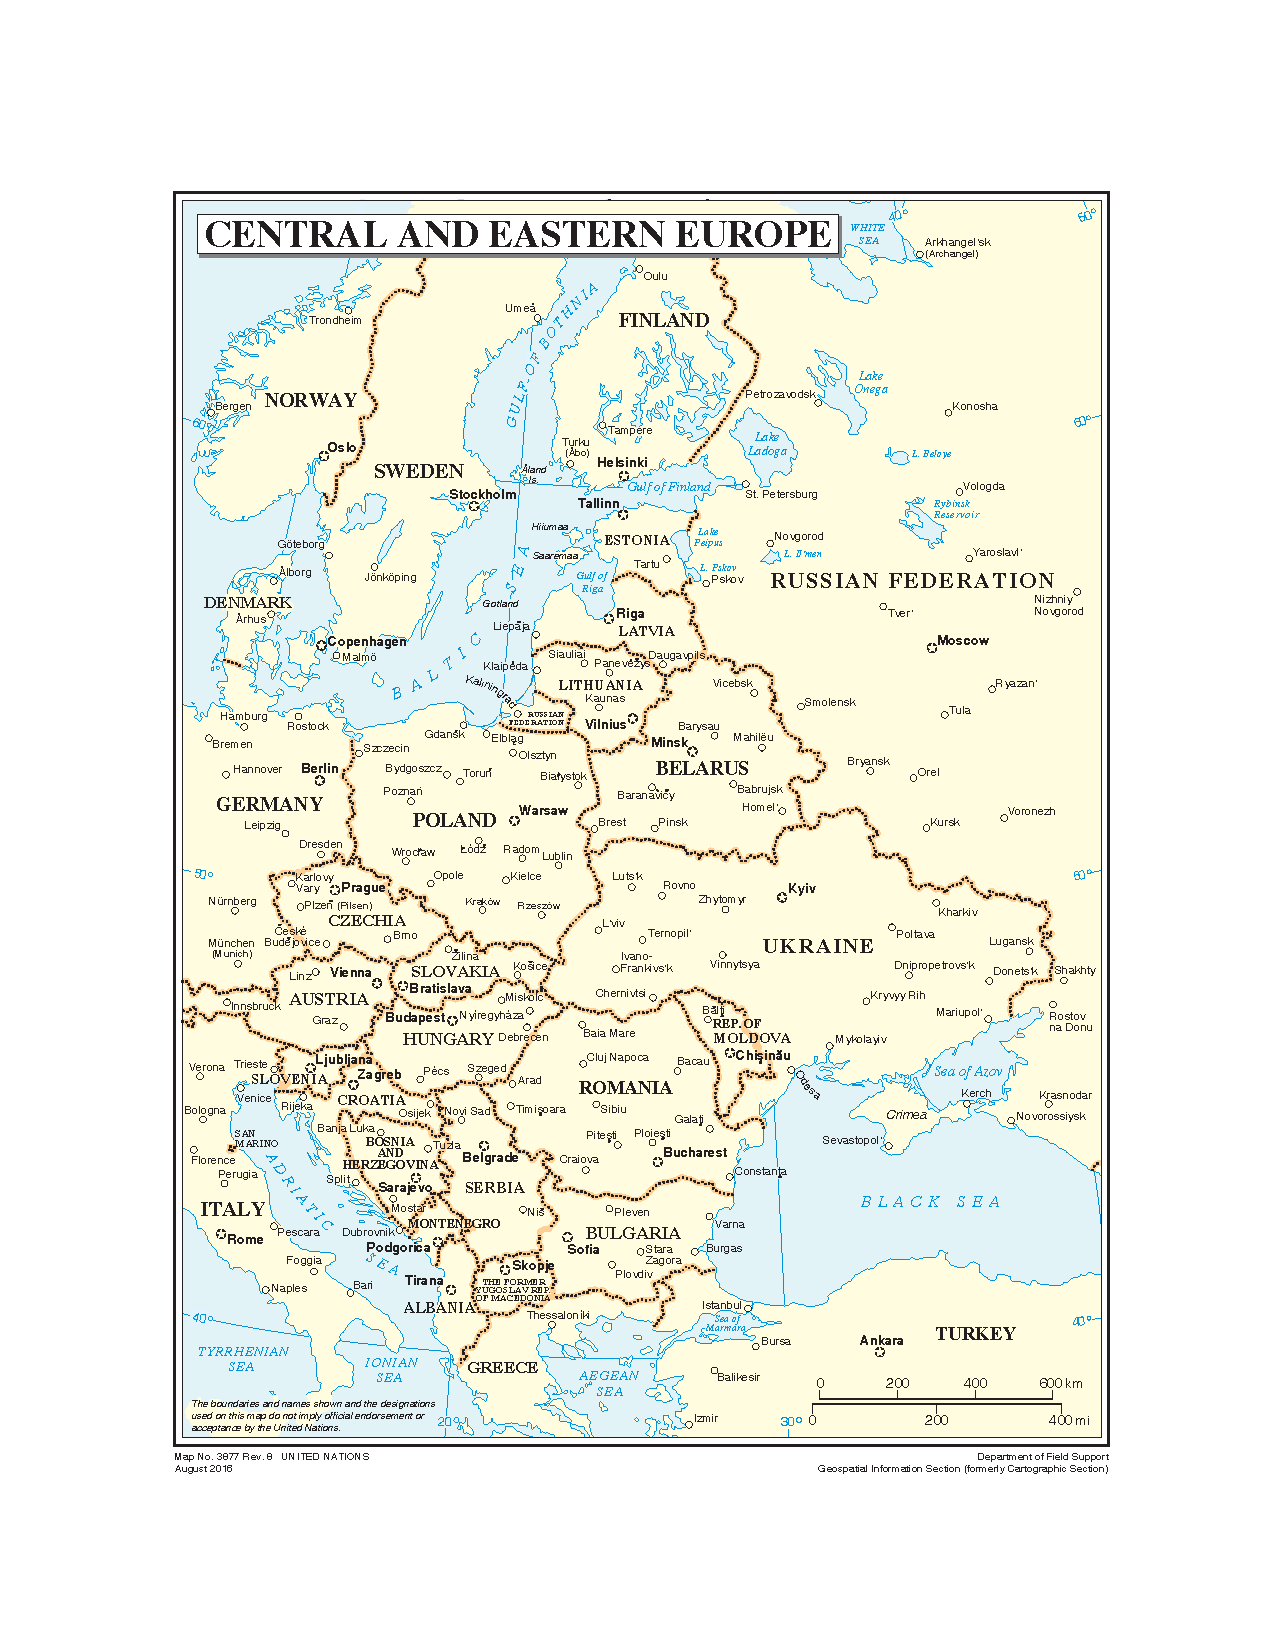
\includegraphics[trim=100 260 370 370, clip, width=.7\textwidth]
                        {\rootdir/img/easteuro}
      \end{column}
      \begin{column}{.4\textwidth}
        \newcommand{\mkCEUMapGraph}[1][]{
  \begin{tikzpicture}[
    every node/.style={draw, circle, inner sep=0pt,
                       text width=1.5em, align=center},
    node IT/.style={},
    node SN/.style={},
    node CR/.style={},
    node H/.style ={},
    node A/.style ={},
    node SK/.style={},
    node CZ/.style={},
    node G/.style ={},
    node P/.style ={},
    #1
    ]

  \node[node IT] (IT) at (0,0)   {IT};
  \node[node SN] (SN) at (1,0)   {SN};
  \node[node CR] (CR) at (2,-1)  {CR};
  \node[node H]  (H)  at (3,0)   {H};
  \node[node A]  (A)  at (1,1)   {A};
  \node[node SK] (SK) at (3,1)   {SK};
  \node[node CZ] (CZ) at (2,2)   {CZ};
  \node[node G]  (G)  at (1,3)   {G};
  \node[node P]  (P)  at (3,3)   {P};

  \draw (G) -- (P);
  \draw (G) -- (CZ);
  \draw (G) -- (A);
  \draw (P) -- (CZ);
  \draw (P) -- (SK);
  \draw (CZ) -- (A);
  \draw (CZ) -- (SK);
  \draw (A) -- (SK);
  \draw (A) -- (H);
  \draw (A) -- (SN);
  \draw (A) -- (IT);
  \draw (SK) -- (H);
  \draw (IT) -- (SN);
  \draw (SN) -- (H);
  \draw (SN) -- (CR);
  \draw (H) -- (CR);

\end{tikzpicture}
}

        \centering
        Graph coloring problem\\ \medskip
        \resizebox{.7\textwidth}{!}{\mkCEUMapGraph}
      \end{column}
    \end{columns}
    \centering \bigskip
    \resizebox{.7\textwidth}{!}{%
    $\xi_2(x,y)= \begin{cases}
      0 & \mbox{if } \exists \text{~edge~} x \leftrightarrow y
                    ~\land \text{~color~} x = \text{color~} y \\
      1 & \text{otherwise}
    \end{cases}
    $}%
  \end{examples}
\end{frame}

% \begin{frame}{CSP Solution Methods}
%   ???
% \end{frame}
